\chapter{Interaction entre atomes de Rydberg sphériques et excitation de gaz dense}
\label{chapter:60s}
%Excitation optique d'atomes de Rydberg à bas $l$ et simulations
\noindent Les premières expériences que nous avons menées sur les interactions entre atomes de Rydberg ont eu lieu dans un nuage dense d'atomes froids au sein duquel sont excités de nombreux atomes vers l'état de Rydberg $\mathrm{60S}$.
Cela permet de mettre en évidence deux aspects différents de l'interaction au sein d'un nuage de Rydberg froid : l'influence des interactions sur la dynamique d'excitation des atomes de Rydberg et le mouvement des atomes en interaction au sein du nuage.

Après un rappel de la forme de l'interaction dipolaire, nous en expliquerons les effets sur le mouvement des atomes de Rydberg dans le nuage et sur la dynamique d'excitation de ces mêmes atomes.
Nous présenterons ensuite une expérience de spectroscopie optique mettant en evidence ces effets.

Le modèle numérique de simulation que nous avons développé nous permettra de confirmer notre compréhension de ces effets et leur importance.
Enfin, nous présenterons une expérience de spectroscopie microonde permettant de sonder plus précisément les énergies d'interactions dans un nuage d'atomes de Rydberg, à différents moments de son expansion.

%\section{Régimes d'excitation en nuage dense : blocage et facilitation}
\section{Les effets de l'interaction dipolaire en nuage dense}


	\subsection{Rappels sur l'interaction dipolaire}
\noindent L'interaction dipolaire entre deux atomes de Rydberg dans le même état $\ket{a}$ et séparés d'une distance $r$ prend la forme suivante, établie en \ref{subsec:interaction_same_level} :
\begin{equation}
\label{eq:Vdd_aa}
\hat{V}_{dd}(r) = \frac{hC_6}{r^6} \cdot \ket{aa}\bra{aa}.
\end{equation}
Ce potentiel d'interaction agit donc comme un simple déplacement de l'énergie de la paire d'atomes par une quantité $E_{int} (r)=hC_6/r^6$ .
Nous travaillerons dans l'hypothèse que cette interaction de Van der Waals est additive pour un ensemble de $N$ atomes.
Ainsi, l'atome $i$ subira la somme des interactions de paire avec les autres atomes $j$ de l'ensemble :
\begin{equation}
\label{eq:Eint_isum}
E_{int}(i) = \sum_{j\neq i} E_{int}(i,j) = \sum_{j\neq i} E_{int}(r_{ij}) = h C_6 \cdot \sum_{j \neq i} \frac{1}{r_{ij}^6}.
\end{equation}
Cette hypothèse d'additivité est valide dès lors que l'on se limite au second ordre du couplage dipôle-dipôle \cite{ENS_CHIPINTERACTION15,MX_TELLER_ADDITIVEVDW}.
La figure \eqref{fig:VdW_sum_N} représente un tel ensemble d'atomes en interaction.
%
\begin{figure}[h]
\centering
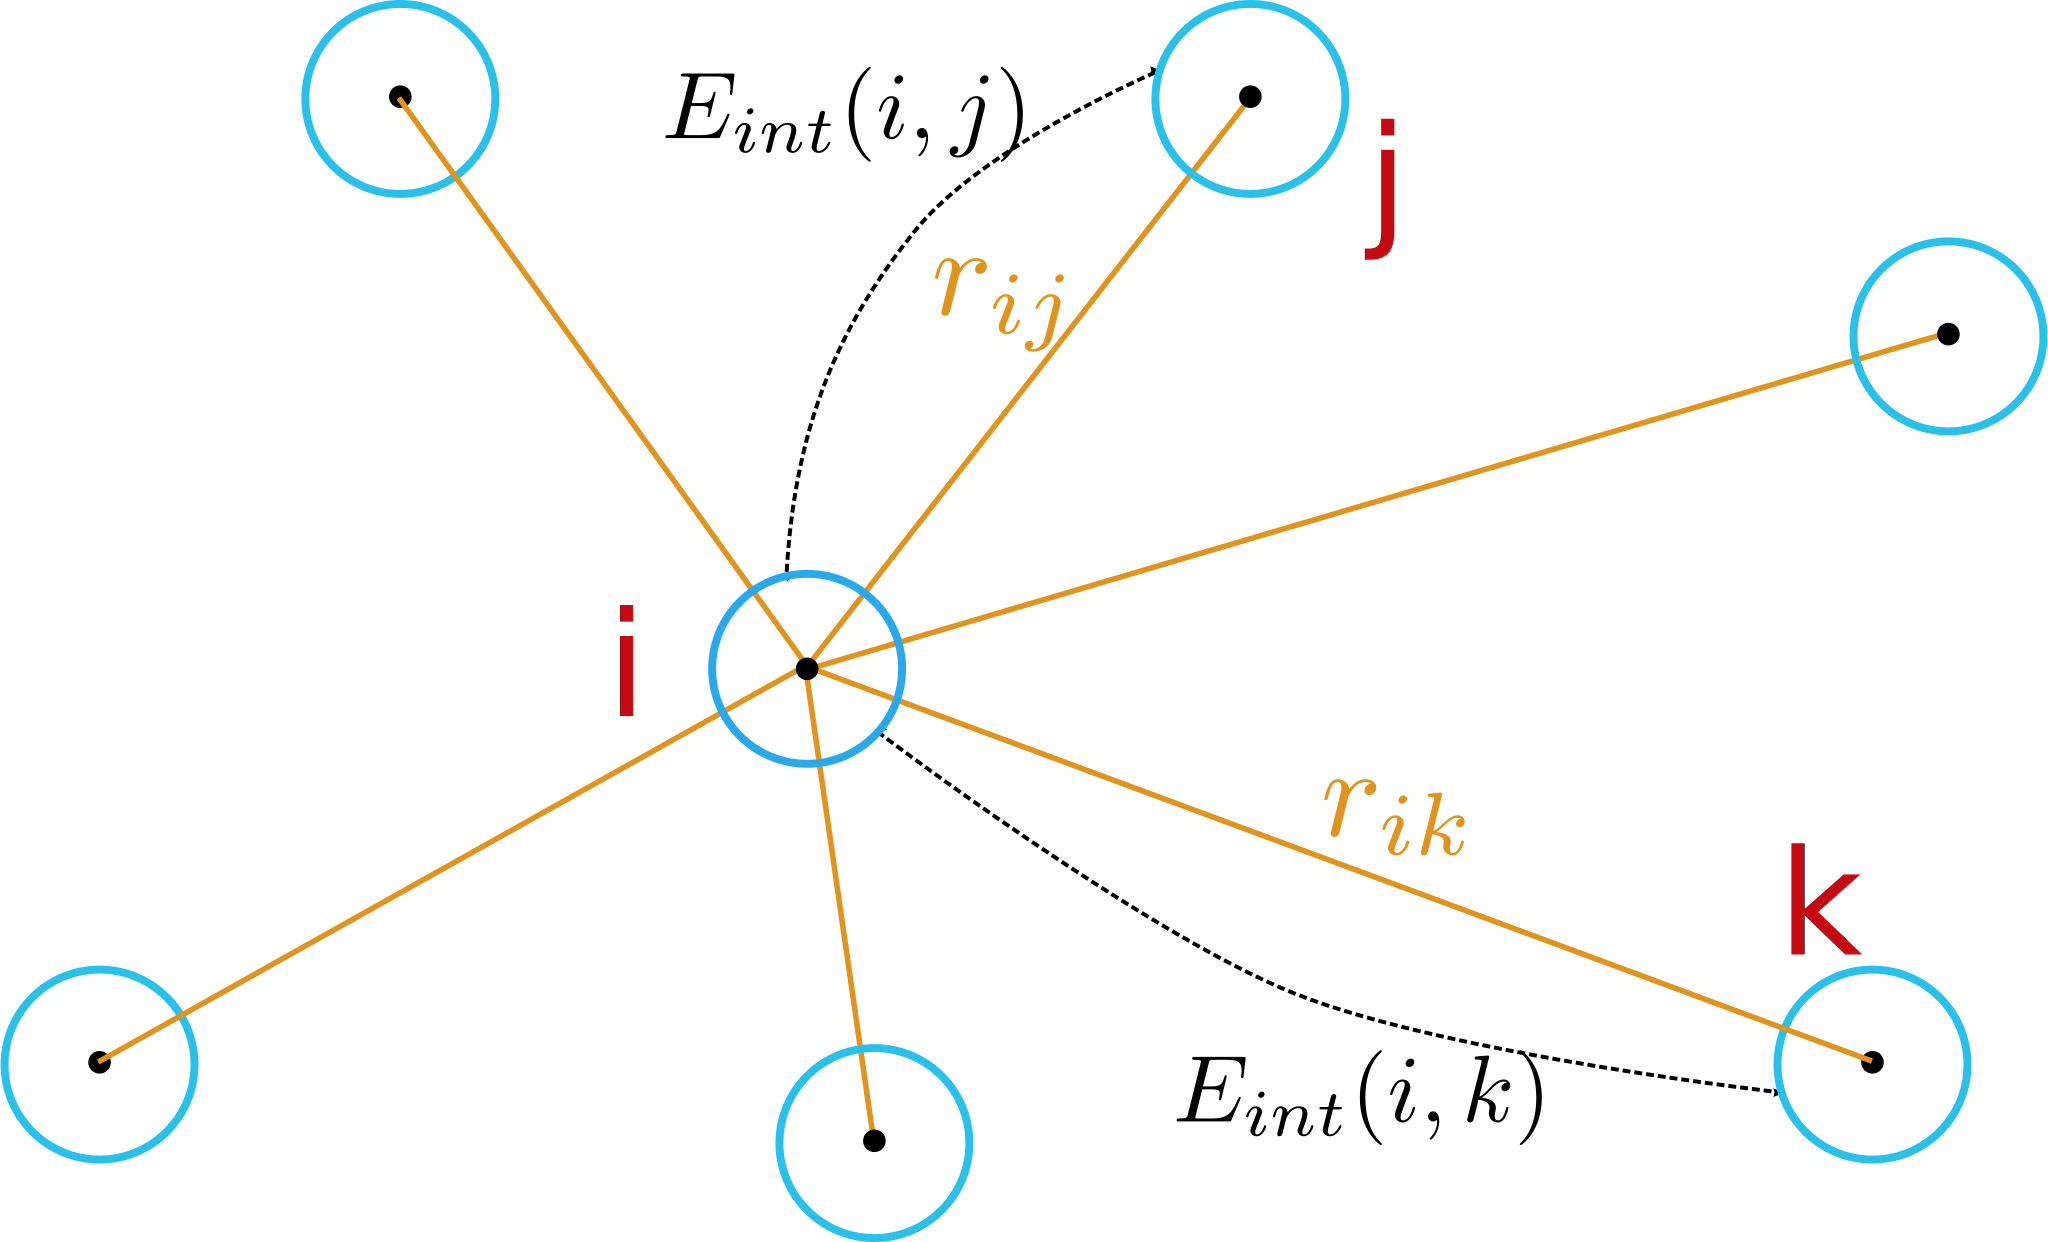
\includegraphics[width=0.6\linewidth]{figures/low_l/Natomes}
\caption[Ensemble de $N$ atomes de Rydberg en interaction Van der Waals]
{Ensemble de $N$ atomes de Rydberg en interaction Van der Waals.
L'énergie d'interaction de chaque atome est la somme de ses énergies d'interaction de paire avec tous les autres.
}
\label{fig:VdW_sum_N}
\end{figure}

	\subsection{Mouvement des atomes au sein d'un gaz dense de Rydberg}
	\noindent Le premier effet des interactions dipolaires au sein d'un nuage d'atomes de Rydberg est un effet mécanique.
Comme nous l'avons vu en \ref{sec:interacting_rydbergs}, l'interaction est répulsive entre atomes de Rydberg dans le même niveau $\ket{\mathrm{nS}}$.
Ainsi, deux atomes de Rydberg en interaction dipolaire subiront chacun une force répulsive, directement dérivée de leur énergie d'interaction,
\begin{equation}
\label{eq:repuls_2atoms}
F = - \frac{d E_{int}}{dr}  = + \frac{6hC_6}{r^7}.
\end{equation}
Cela équivaut à un traitement classique de l'effet mécanique de l'interaction dipolaire, bien que le calcul de cette même interaction ne le soit pas.
Cela nous est permis par la forme simple de l'interaction dipolaire entre deux atomes dans le même état de Rydberg, donnée par l'équation \eqref{eq:Vdd_aa}, qui consiste en un simple déplacement d'énergie du niveau de paire $\ket{aa}$.

Prenons l'exemple de deux atomes dans le niveau $\mathrm{60S}$, séparés d'une distance de $\SI{5}{\um}$ : leur énergie d'interaction vaut $hC_6/r^6 = h\cdot {\SI{137.6}{\GHz\raiseto{6}\um}}/(\SI{5}{\um})^6 = \SI{8.8}{\MHz}$.
Ils se repoussent donc avec une force valant %$6hC_6/r^7 = 6h\cdot \SI{137.6}{\GHz\raiseto{6}\um}/(\SI{5}{\um})^7 = \SI{6.97e-27}{\mega\newton} = \SI{6.97e-21}{\newton}$.
$6hC_6/r^7 =\SI{6.97e-21}{\newton}$.
Étant donnée la masse du rubidium, cette force répulsive correspond à une accélération valant $F/m_{Rb87} = \SI{4.83e4}{\m\per\s\squared}$, soit $\num{5000}$ fois plus que l'accélération de la gravité.
Une intégration numérique grossière permet d'extraire un ordre de grandeur du déplacement des atomes : en $\SI{20}{\us}$, ils auront presque atteint leur vitesse relative maximale de $\SI{0.284}{\m\per\s}$ et en $\SI{10}{\us}$ seulement la distance qui les sépare aura augmenté de $\SI{1.75}{\um}$.
Leur énergie d'interaction aura par là chuté d'un facteur $\SI{5.77}{}$, ce qui constitue une modification considérable du système.

La généralisation à $N$ atomes se fait en additionnant vectoriellement les forces répulsives dues à chaque interaction de paire :
\begin{equation}
\label{eq:repuls_Natomes}
\vec{F}(i) =  \sum_{j\neq i} -\vec{\nabla}E_{int}(i,j)
= \sum_{j\neq i} \frac{6hC_6}{r_{ij}^7} \cdot \frac{-\vec{r}_{ij}}{r_{ij}}
= - 6hC_6 \cdot \sum_{j\neq i} \frac{\vec{r}_{ij}}{r_{ij}^8}.
\end{equation}
%
Cette force répulsive décroît très vite avec la distance.
On s'attend ainsi à ce que deux atomes de Rydberg en interaction s'accélère mutuellement pendant un temps court, se propageant ensuite balistiquement dans des directions opposées.
C'est ce que confirme l'exemple de la paire $\ket{\mathrm{60S,60S}}$ précédemment cité.
Il est intéressant de noter qu'au sein d'un nuage d'atomes de Rydberg, les atomes du c\oe ur  sont repoussés par les interactions dipolaires de tous les côtés.
Les atomes du bord du nuage seront alors expulsés en premier, puis petit à petit les atomes plus au centre pourront commencer à se déplacer.
Le nuage subit ainsi une expansion hydrodynamique non triviale, que nous mesurerons expérimentalement et simulerons numériquement.

	\subsection{Deux régimes d'excitation en interaction dipolaire forte}\label{subsec:excitation_bloc_facil}
	%Le blocage dipolaire et la facilitation}

\noindent Les interactions dipolaires ont également une influence importante sur l'excitation d'un ensemble dense d'atomes de Rydberg.	
En effet, la présence d'un atome de Rydberg conditionne l'excitation ultérieure d'autres atomes de Rydberg dans son voisinage.
Lorsque l'excitation est faite à résonance, cet effet est connu sous le nom de \og blocage dipolaire \fg{}.

	\subsubsection*{Blocage dipolaire et super-atomes}
\noindent Le mécanisme du blocage dipolaire est illustré en figure (\ref{fig:dip_block} a)).
Considérons deux atomes dans l'état fondamental $\ket{g}$, séparés d'une distance $r$.
L'état de la paire est alors $\ket{g,g}$.
Un laser est accordé à résonance pour exciter l'un quelconque de ces deux atomes vers le niveau de Rydberg $\ket{ry}$.
L'état de la paire devient ainsi $\ket{g,ry}$.% ou $\ket{ry,g}$.
Si l'on souhaite exciter le second atome vers le niveau $\ket{ry}$, alors il faut considérer l'énergie nécessaire à la transition $\ket{g,ry} \rightarrow \ket{ry,ry}$.
Or ce dernier état de paire subit un déplacement d'énergie dû à l'interaction de Van der Waals
%
\begin{equation}
\label{eq:DeltaE_block}
\Delta E_{\ket{ry,ry}}(r) = E_{\ket{ry,ry}}(r)-E_{\ket{ry,ry}}(\infty)
= E_{int}(r).
\end{equation}
%
Le laser, qui était à résonance avec la transition $\ket{g,g}\rightarrow\ket{g,ry}$, n'est ainsi plus à résonance avec la transition $\ket{g,ry}\rightarrow\ket{ry,ry}$.
L'excitation du second atome vers un niveau de Rydberg s'en trouve bloquée.

\begin{figure}[!h]
\centering
\includegraphics[height=.3\textheight]{figures/low_l/dip_block}
\caption[Mécanisme du blocage dipolaire]{
Illustration du mécanisme de blocage dipolaire.
\textbf{a)} Diagramme d'énergie des niveaux de paire à zéro, un ou deux atomes excités, en fonction de la distance interatomique $r$.
$\ket{g}$ est le niveau fondamental et $\ket{ry}$ le niveau de Rydberg considéré.
Aux courtes distances, l'interaction dipolaire déplace l'excitation du deuxième atome vers le niveau de Rydberg hors de résonance avec le laser ayant excité le premier atome.
$\gamma$ représente la largeur spectrale de la raie d'excitation à un atome, $E_{int}$ l'énergie d'interaction entre deux atomes de Rydberg et $r_b$ le \og rayon de blocage \fg{}.
\textbf{b)} Généralisation à un ensemble d'atomes. Les points bleus sont des atomes dans l'état fondamental et les points rouges sont des atomes de Rydberg.
Le mécanisme de blocage empêche l'excitation de deux atomes de Rydberg dans un même sphère de rayon $r_b$, représentée par les disques rouges.
}
\label{fig:dip_block}
\end{figure}

Le laser d'excitation n'est pas infiniment fin spectralement et l'effet de blocage dipolaire sera limité par sa largeur spectrale.
On peut en effet considérer que le laser est résonant avec la transition dès lors que le désaccord entre eux est inférieur à la demi-largeur spectrale $\gamma/2$ de la raie d'excitation.
Nous définirons ainsi le \og rayon de blocage \fg{} $r_b$ comme étant la distance en-deçà de laquelle le désaccord est supérieur à la demi-largeur spectrale :
\begin{equation}
\label{eq:def_rayon_bloc}
\Delta E_{int}(r_b) = \gamma /2 
\end{equation}
%
Dans le cas qui nous intéresse, l'interaction dipolaire a une forme de Van der Waals en $1/^6$, permettant de réécrire l'équation \eqref{eq:def_rayon_bloc} sous la forme
\begin{equation}
\label{eq:def_rayon_bloc}
\frac{C_6}{r^6} = \gamma /2 \text{ , soit } r_b = \sqrt[6]{\frac{C_6}{\gamma /2}}
\end{equation}
%
Le mécanisme de blocage est donc effectif à l'intérieur d'un \og volume de blocage\fg{} autour de chaque atome de Rydberg déjà excité.
Ce volume de blocage est une sphère de rayon $r_b$, représentée en figure (\ref{fig:dip_block} b)).

Revenons au cas de deux atomes :
il existe deux états de paire à une excitation, qui sont $\ket{g,ry}$ et $\ket{ry,g}$.
Ces deux états sont dégénérés et le laser couple le niveau fondamental $\ket{g,g}$ indifféremment à $\ket{g,ry}$ et à $\ket{ry,g}$, avec même une fréquence de Rabi $\Omega$.
La combinaison symétrique $\ket{D} = \left( \ket{g,ry} + \ket{ry,g} \right) / \sqrt{2}$, appelée état collectif de Dicke des deux atomes, est alors couplée à l'état fondamental avec une fréquence de Rabi augmentée $\Omega\sqrt{2}$.
Ce facteur d'accroissement a été mis en évidence expérimentalement par le groupe de A. Browaeys et P. Grangier \cite{MX_BROWAEYS_COLLECRABIBLOCK}, en observant deux atomes piégés dans des pinces optiques.

L'idée se généralise au cas à $N$ atomes en utilisant encore une fois le modèle de Dicke.
Dans un rayon de blocage contenant $N_b$ atomes, l'état du système oscille entre l'état fondamental et l'état de Dicke à une excitation, toute excitation supplémentaire étant interdite par blocage dipolaire.
Cette oscillation se fait cette fois avec une fréquence de Rabi $\Omega\sqrt{N_b}$.
Un modèle simple de ce phénomène consiste à voir l'ensemble de ces $N_b$ atomes comme un unique \og super-atome \fg{} ayant un moment de transition dipolaire $\sqrt{N_b}$ plus grand  que celui d'un atome isolé.
Ce modèle de super-atome a été exploité avec succès pour expliquer des observations expérimentales par les groupes d'I. Bloch \cite{MX_BLOCH_SUPERATOM} et de H. Ott \cite{MX_OTT_SUPERATOM}.


	\subsubsection*{Excitation facilitée et agrégats de Rydberg}
	
\noindent Dans le régime de blocage dipolaire, l'interaction entre atomes de Rydberg désaccorde toute excitation supplémentaire au voisinage d'un premier atome de Rydberg.
On peut alors imaginer décaler la fréquence du laser d'excitation de façon à compenser ce désaccord et ainsi retrouver une condition de résonance.

Reprenons le cas de deux atomes présenté ci-dessus en figure \eqref{fig:dip_block}.
Considérons cette fois un laser désaccordé de $\Delta$ par rapport à la transition $\ket{g,g} \rightarrow \ket{g,ry}$.
Le premier atome pourra toujours être excité hors résonance par le laser désaccordé.
Le second atome sera ensuite excité, à résonance, si la condition
\begin{equation}
\label{eq:condition_facil}
\Delta = E_{int}(r)/h = \frac{C_6}{r^6}
\end{equation}
est satisfaite.
\`A un désaccord laser $\Delta$ fixé correspond ainsi un \og rayon de facilitation \fg{}, défini par
\begin{equation}
\label{eq:r_facil}
r_f = \sqrt[6]{\frac{C_6}{\Delta}}.
\end{equation}
En raison de la largeur spectrale $\gamma$ du laser, l'excitation du second atome de Rydberg est donc \og facilitée \fg{} par la présence du premier, dès lors qu'ils sont séparés d'une distance $r_f \pm \delta r_f$,
où $\delta r_f = \frac{1}{2} \left( \sqrt[6]{C_6/(\Delta-\gamma/2)} - \sqrt[6]{C_6/(\Delta+\gamma/2)} \right)$, soit $\delta r_f \simeq r_f \gamma / (3\Delta)$ au premier ordre en $\gamma / \Delta$.
La figure (\ref{fig:dip_facil} a) )représente ce mécanisme d'\og excitation facilitée \fg{} .
%	
\begin{figure}[!h]
\centering
\includegraphics[height=.3\textheight]{figures/low_l/dip_facil}
\caption[Mécanisme de d'excitation facilitée]{
Mécanisme de d'excitation facilitée.
\textbf{a)} Diagramme d'énergie des niveaux de paire à zéro, une ou deux atomes excités, en fonction de la distance interatomique $r$.
Le premier atome de Rydberg est excité hors résonance.
Le désaccord $\Delta$ du laser permet de compenser l'interaction dipolaire à la distance $r_f$ et d'exciter à résonance le second atome.
\textbf{b) - e)} Évolution dans le temps d'un agrégat de Rydberg.
Les points bleus représentent l'ensemble de départ d'atomes dans l'état fondamentalet les points rouges représentent les atomes de Rydberg.
Les bandes vertes représentent les régions \og facilitées \fg{} définies par l'équation \eqref{eq:facil_Natomes} où de nouveaux atomes de Rydberg peuvent être excités à résonance.
}
\label{fig:dip_facil}
\end{figure}

Au sein d'un ensemble d'atomes, chacun a une probabilité égale d'être le premier atome excité, hors résonance, vers un niveau de Rydberg.
Dès lors que ce premier atome de Rydberg est excité, l'excitation est facilitée pour les atomes qui sont à une distance $r_f$ de celui-ci, vérifiant par-là la condition \eqref{eq:r_facil}.
L'excitation facilitée continue ainsi de proche en proche, tant qu'il existe un atome $i$ satisfaisant
\begin{equation}
\label{eq:facil_Natomes}
\Delta = \sum_{j\neq i} {\frac{C_6}{r_{ij}}},
\end{equation}
où la somme est faite sur tous les atomes de Rydberg $j$ déjà excités, situés chacun à distance $r_{ij}$ de l'atome $i$.

Le phénomène de blocage dipolaire est remplacé ici par la formation rapide d'un \og agrégat de Rydberg \fg{} fortement corrélé, autour du premer atome de Rydberg, la \og graine \fg{} de cet agrégat.
Les distances relatives entre atomes de Rydberg sont déterminées par l'équation\eqref{eq:facil_Natomes} et donc contrôlées par le désaccord $\Delta$ du laser d'excitation.
La figure (\ref{fig:dip_facil} b)-e)) représente cette excitation séquentielle facilitée d'un agrégat de Rydberg.
%
%\newpage
%		\noindent les deux régimes d'excitation déterminée par les interactions :\\
%		explication du blocage dipolaire, et des effets qui le limitent (ailes de la gaussienne du nuage) \\
%		pourquoi c'est difficile dans un BEC : mention du Pfau shift \\
%		mention de la négligeabilité des excitations de paires ?

\section{Observation expérimentale des interactions}
\noindent Afin de mettre en évidence les effets des interactions dipolaires, nous avons mené deux expériences complémentaires.
En premier lieu, la spectroscopie optique du nuage permet de s'intéresser à l'excitation sous blocage dipolaire fort et à l'excitation facilitée à désaccord positif.
Ensuite, la spectroscopie microonde du nuage, à différents délais après l'excitation laser, permet de sonder la distribution des énergies d'interaction au sein du nuage au cours de son expansion.
Ces expériences sont discutées en détail dans la thèse de Raul Celistrino Teixeira \cite{PHD_CELISTRINO}.

	\subsection{Spectroscopie optique du nuage : différents régimes d'excitation}\label{subsec:optical_spectra}
	\subsubsection*{Conditions de l'expérience}
\noindent	L'expérience de spectroscopie optique visse à observer l'excitation des atomes de Rydberg sous l'influence des interactions dipolaires, dans les régimes de blocage et d'excitation facilitée.
Cela nécessite, entre autres, un nuage d'atomes dans l'état fondamental suffisamment dense afin que la condition de facilitation \eqref{eq:facil_Natomes} puisse être satisfaite.
Cependant, une forte densité d'atomes dans l'état fondamental risque d'interférer avec l'excitation de Rydberg, indépendamment des interactions dipolaires.
En effet, l'électron de Rydberg, qui est presque libre, est sensible à cette densité atomique.
En première approximation, l'interaction entre l'électron de Rydberg et les atomes dans l'état fondamental prend la forme d'un dplacement d'énergie $V_e$ proportionnel à la densité atomique moyenne $\bar{\rho}$ \cite{MX_PFAURYDBERGBEC13} :
\begin{equation}
\label{eq:Pfau_shift}
V_e = \frac{2\pi \hbar ^2 a_s}{m_e} \bar{\rho},
\end{equation}
où $a_s$ est la longueur de diffusion caractérisant la force de l'interaction.
Le groupe de T. Pfau a mis en évidence cette interaction et obtenu une longueur de diffusion pour le \Rb{87} valant $a_s = -\SI{16.1}{}~a_0~$, indépendante du nombre quantique principal $n$ \cite{MX_PFAURYDBERGBEC13}.
%Le potentiel d'interaction $V_e$ étant négatif, nous avons ici affaire à une interaction qui abaisse l'énergie des niveaux de Rydberg.
Dans un condensat de Bose-Einstein avec une densité atomique typique de $\SI{e13}{\per \raiseto{3}\centi\meter}$, l'énergie d'interaction est de l'ordre de $V_e/h = -\SI{1}{\MHz}$.
Dans ce cas, nous serions en présence de deux interactions antagoniste de même ordre de grandeur : l'interaction dipôle-dipôle répulsive, qui augmente l'énergie des niveaux de Rydberg et l'interaction de l'électron de Rydberg avec les atomes dans l'état fondamental, qui abaisse l'énergie des niveaux de Rydberg.
Cela aurait pour effet de réduire le rayon de blocage, qui dépend directement de la largeur spectrale de l'excitation sans interaction dipolaire.

Il nous a fallu trouver une densité atomique permettant l'observation de l'excitation facilitée et du blocage dipolaire, tout en limitant l'effet d'interaction de l'électron de Rydberg avec les atomes dans l'état fondamental.
La spectroscopie optique de l'excitation de Rydberg a été faite dans un nuage thermique froid et non dans un condensat de Bose Einstein.
Ce nuage comporte $\SI{12000}{} \pm \SI{1000}{}$ atomes, piégés magnétiquement à environ $\SI{210}{\um}$ de la puce atomique.
Le piège prend une forme très allongée dans la direction $x$, et les atomes sont refroidis à une température de $\SI{500}{} \pm \SI{150}{\nano\kelvin}$.
Le profil de densité atomique est alors gaussien dans les trois directions, avec des rayons à $e^{-1/2}$ valant respectivement $(\sigma_x;\sigma_y;\sigma_z) = (\num{23.2} ; \num{4.5} ; \num{4.2})\si{\um}$.
La densité au centre vaut ici $n_0 = \num{1.7}\pm\SI{0.15}{\per\raiseto{3}\cm}$.
Cela limite l'interaction de l'électron de Rydberg avec les atomes dans l'état fondamental à une énergie $V_e = -\SI{168}{\kHz}$, très inférieure à la largeur spectrale d'excitation à un atome, estimée \footnote{
Cette valeur est extraite de l'ajustement gaussien d'un spectre d'excitation optique dans un piège dilué et à faible excitation, donc sans interactions dipolaires.
Ce spectre est présenté comme référence en figure \eqref{fig:data_spectresoptiques}.}
à $2\gamma = \SI{626}{\kHz}$.
La contribution de cette interaction pourra ainsi être négligée dans la suite de notre discussion.


		\subsubsection*{Résultats expérimentaux}
\noindent Les spectres d'excitation du niveau de Rydberg $\mathrm{60S}$ depuis le niveau fondamental $\mathrm{5S}$, obtenus pour différentes durées d'impulsion laser, sont représentés en figure \eqref{fig:data_spectresoptiques}.
Le graphe représente aussi un spectre d'excitation dans un nuage dilué et à faible taux d'excitation, servant de spectre de référence sans interactions.
%
\begin{figure}[!h]
\centering
\includegraphics[width=.85\linewidth]{figures/low_l/data_spectres_optiques}
\caption[Spectres optiques d'excitation en régime d'interaction dipolaire forte]{Spectres optiques d'excitation en régime d'interaction dipolaire forte.
L'excitation est réalisée à différentes durées d'impulsion laser : $\SI{2}{}$, $\SI{20}{}$, $\SI{50}{}$ et $\SI{100}{\us}$.
La courbe magenta est un spectre de référence sans interaction, représenté avec une échelle différente (échelle de droite).
Les pics d'excitation autour de $\Delta = \SI{20}{\MHz}$ sont dûs à la modulation en fréquence du laser, nécessaire à sa stabilisation par un dispositif Pound-Drever-Hall.
}
\label{fig:data_spectresoptiques}
\end{figure}
%
Un élargissement vers les hautes fréquences apparaît très clairement dès les faibles temps d'excitation.
Cet élargissement est caractéristique de l'excitation facilitée par interactions :
une fois le premier atome de Rydberg excité, un agrégat se forme rapidement autour et permet d'amplifier largement l'excitation à désaccord positif.
Plus le désaccord est élevé cependant, plus longtemps se fera attendre cette première excitation, ce qui explique l'élargissement de plus en plus prononcé aux temps d'impulsion longs.

Cela se voit très bien sur les graphes de la figure \eqref{fig:data_saturoptique}, qui représente l'évolution du nombre d'atomes de Rydberg excité en fonction de la durée d'impulsion laser, pour différents désaccords.
%
\begin{figure}[!h]
\centering
\includegraphics[width=.7\linewidth]{figures/low_l/satur_spectres_optiques_extract}
\caption[Saturation de l'excitation optique en régime d'interaction dipolaire forte]{Saturation de l'excitation optique en régime d'interaction dipolaire forte.
Évolution du nombre d'atomes de Rydberg en fonction de la durée d'impulsion laser, pour différents désaccords : $\SI{0}{}$, $\SI{2}{}$, $\SI{4}{}$, $\SI{8}{}$ et $\SI{10}{MHz}$.
Les données sont extraites des spectres de la figure \eqref{fig:data_spectresoptiques}.
}
\label{fig:data_saturoptique}
\end{figure}
%
On y remarque effectivement qu'à grand désaccord, le nombre d'atome de Rydberg présente un effet de seuil correspondant à l'excitation non résonante de la \og graine \fg{}.

Le comportement à résonance montre une croissance rapide du nombre d'atomes excités dans les premiers instants, puis une augmentation plus lente.
En effet, le centre nuage est saturé de super-atomes en régime de blocage fort dès les premières microsecondes.
Ensuite, de nouveaux atomes de Rydberg sont excités dans les ailes peu denses du nuage.
Celles-ci contiennent beaucoup moins d'atomes dans l'état fondamental d'une part, et le laser bleu y est moins intense d'autre part.
Ces deux facteurs contribuent à ralentir fortement la dynamique d'excitation dans ces régions-là.
Enfin, le mouvement d'expansion du nuage de Rydberg dû aux interactions éloigne les super-atomes les uns des autres au centre du nuage, où de nouvelles excitations deviennent possibles après quelques dizaines de microsecondes.
Cela explique pourquoi le nombre d'atomes de Rydberg continue d'augmenter, contrairement aux prédictions de l'approximation du \og gaz gelé \fg{}.% communément utilisée.

	\subsection{Spectroscopie microonde : une sonde pour l'énergie d'interaction}
\noindent Afin de mieux comprendre le mouvement au sein du nuage de Rydberg, nous avons réalisé la spectroscopie de la transition $\mathrm{60S} \rightarrow \mathrm{57S}$ dans différentes conditions.
Nous présentons ici le principe de cet outil de spectroscopie microonde comme sonde des énergies d'interaction dans le nuage, et les expériences que nous avons menées.

	\subsubsection*{Principe de la spectroscopie microonde et choix de la transition}
\noindent Comme nous l'avons vu au chapitre \ref{chapter:Rydberg}, les différents niveaux de Rydberg sont affectés différemment par les interactions dipolaires.
En particulier, dans le régime de Van der Waals, cela se traduit par des coefficients de Van der Waals $C_6$ différents.
Ainsi, le niveau $nS$ et le niveau $n'S$ verront leur énergie déplacée de quantités différentes pour une même distance inter-atomique.
En conséquences, les fréquences de transition entre niveaux de Rydberg seront décalées.
Sonder ces décalages de fréquence, c'est-à-dire faire la spectroscopie de telles transitions, nous renseignera sur la distribution des énergies d'interaction au sein du nuage.
Idéalement, un seul atome du nuage sera transféré vers un autre niveau de Rydberg, et la fréquence de cette transition nous renseignera sur l'énergie d'interaction de cet atome avec tous ses voisins.

Cela requiert cependant un choix attentif du niveau vers lequel seront transférés les atomes de Rydberg.
En premier lieu, les niveaux $P$ sont à éviter.
La branche attractive de l'interaction $nS - n'P$ mène à une ionisation de Penning des atomes de Rydberg : l'atome dans le niveau $nS$ et l'atome dans le niveau $n'P$ s'attirent l'un l'autre, et s'ionisent mutuellement lorsqu'ils sont trop proches.
Nous restreindrons donc notre choix aux niveaux $n'S$ voisins du $\mathrm{60S}$, accessibles par des transitions à deux photons.

Pour une paire d'atomes séparés de $r$, l'interaction $\mathrm{60S}-n'S$ prend la forme de l'équation \eqref{eq:MatrixCab_Aab} :
\begin{equation}
\label{eq:Matrix_60SnS}
V_{eff}/h = \bordermatrix{~ 	&\ket{\mathrm{60S-n'S}} 	& \ket{\mathrm{n'S-60S}} \cr
	\bra{\mathrm{60S-n'S}}		&C_{6,\mathrm{60S-n'S}}		&A_{6,\mathrm{60S-n'S}}	\cr 
	\bra{\mathrm{n'S-60S}} 		&A_{6,\mathrm{60S-n'S}}		&C_{6,\mathrm{60S-n'S}} \cr} \ \cdot \frac{1}{r^6},
\end{equation}
%
où $C_6$ et $A_6$ sont les coefficients de Van der Waals pour l'interaction directe et pour l'interaction d'échange respectivement.
Les états $\ket{\mathrm{60S-n'S}}$ et $\ket{\mathrm{n'S-60S}}$ sont dégénérés et séparés en leurs combinaisons symétrique et antisymétrique, $(\ket{\mathrm{60S-n'S}}\pm\ket{\mathrm{n'S-60S}})/\sqrt{2}$.
Ces deux états propres sont déplacés d'une énergie $h\cdot (C_{6,60S-n'S} \pm A_{6,60S-n'S}) / r^6$.
Cette structure de niveaux est représentée en figure (\ref{fig:60S-nS} a)).
%
\begin{figure}[h]
\centering
\includegraphics[width=\linewidth]{figures/low_l/60S-nS}
\caption[Structure de niveau 60S-nS sous interaction dipolaire]{
Structure de niveau 60S-nS sous interaction dipolaire
\textbf{a)} La paire $\mathrm{60S-nS}$ est déplacée en énergie par le terme d'interaction directe $C_{6,\mathrm{60SnS}}/r^6$ et ses deux états dégénérés sont séparés par l'interaction d'échange, avec un écart d'énergie de $2A_{6,60SnS}/r^6$.
\textbf{b)} Diagramme d'énergie d'une paire dans les niveaux $\mathrm{60S-60S}$ et $\mathrm{60S-57S}$.
Le terme d'échange $A_{6,\mathrm{60S-57S}}$ étant quasi-nul, la dégénérescence des niveaux de paire $\ket{\mathrm{60S,57S}}$ et $\ket{\mathrm{57S,60S}}$ n'est pas levée et la paire se comporte comme un système à deux niveaux.
La transition entre ces deux niveaux est déplacée par les interactions dipolaires.
}
\label{fig:60S-nS}
\end{figure}
%
La levée de dégénérescence des niveaux de paire engendre des spectres à deux raies de transition, séparées en fréquence de $2A_{6,\mathrm{60S-nS}}/r^6$.
Si l'on y ajoute un troisième atome de Rydberg, il y a alors trois paires en interaction, ce qui complexifie d'autant plus la structure de niveaux et le spectre de la transition.
En fin de compte, au sein d'un ensemble de $N$ atomes de Rydberg dans le niveau $\mathrm{60S}$, une  excitation du niveau $n'S$ sera délocalisée sur des états propres à $N$ atomes.
Ces états propres sont des combinaisons linéaires de la base séparable $\{\ket{i} = 
\ket{\mathrm{60S}}_1\otimes\dots\otimes\ket{n'S}_i\otimes\dots\otimes\ket{\mathrm{60S}}_N$,
%\ket{1=\mathrm{60S},\dots,i=n'S,\dots,N=\mathrm{60S}} \}_{i=1\text{ à } N}$
très dépendantes de la configuration du nuage.
Plus la base des états propres à une excitation est différente de la base des $\ket{i}$, plus le spectre d'excitation devient difficile à relier aux énergies d'interaction.

Le niveau $n'S$ idéal serait donc celui pour lequel les états propres à une excitation sont ceux où l'excitation est localisée sur un atome.
Pour cela, le terme d'échange $A_6$, responsable de la délocalisation de l'excitation, doit être le plus petit possible, c'est-à-dire très petit devant $C_6$.
La table \eqref{tab:VdW-60SnS} répertorie les coefficients de Van der Waals $C_{6,\mathrm{60S-n'S}}$ et $A_{6,\mathrm{60S-n'S}}$ pour les niveaux $n'S$ proches du $\mathrm{60S}$.
%
\begin{table}[!h]
	\centering
	\caption[Coefficients de Van der Waals pour différents niveaux $60S-n'S$]{Coefficients de Van der Waals pour différents niveaux $60S-n'S$
	}
	\label{tab:VdW-60SnS}
	\begin{tabular}{c c c}
		\toprule\midrule
		~
		& $C_{6,60S-n'S}$
		& $A_{6,60S-n'S}$\\		
		~
		& $(\si{\GHz\raiseto{6}\um})$
		& $(\si{\GHz\raiseto{6}\um})$\\
		\midrule
		60S-63S & \SI{-89.26}{} & \SI{0.61}{} \\
		60S-62S & \SI{-411.36}{} & \SI{14.96}{} \\
		60S-61S & \SI{292.25}{} & \SI{248.60}{} \\
		60S-60S & \SI{137.62}{} & \SI{}{} \\
		60S-59S & \SI{245.13}{} & \SI{209.55}{} \\
		60S-58S & \SI{-209.26}{} & \SI{7.77}{} \\
		60S-57S & \SI{-43.67}{} & \SI{0.30}{} \\
		\midrule
		\bottomrule
 	\end{tabular}
\end{table}
%
On y trouve les niveaux $\mathrm{63S}$ et $\mathrm{57S}$, qui présentent des termes d'échanges avec le $\mathrm{60S}$ petits devant les termes d'interaction directe ($C_6 / A_6 \sim 150$).
Étant donné le caractère attractif de l'interaction directe pour les paires $\mathrm{60S-57S}$ et $\mathrm{60S-63S}$, il est préférable de choisir la plus petite de ces interactions afin de limiter le processus d'ionisation de Penning que nous décrivions pour les paires $nS-n'P$.

Nous choisirons donc, pour faire la spectroscopie microonde du nuage de Rydberg, la transition $\mathrm{60S-57}$.
Nous disposerons ainsi d'un diagramme de niveaux simple, représenté pour deux atomes en figure (\ref{fig:60S-nS} b)), fournissant un système effectif à deux niveaux.
Lorsque les deux atomes n'interagissent pas, la transition à deux photons du niveau de paire $\ket{\mathrm{60S,60S}}$ vers les niveaux de paire dégénérés $\ket{\mathrm{57S,60S}}$ et $\ket{\mathrm{60S,57S}}$ se fait à une fréquence $\nu_0 = 2\times \SI{58.229}{\GHz}$.
En présence d'interactions, la transition est déplacée d'une quantité
\begin{equation}
\label{eq:60s-57s_2atoms}
\Delta\nu (r) = \frac{C_{6,60S60S}-C_{6,60S-57S}}{r^6} = \eta \frac{C_{6,60S60S}}{r^6},
\end{equation}
avec $\eta = \num{1.317}$.

La généralisation à un ensemble de $N$ atomes de Rydberg se fait dans l'hypothèse d'additivité des interactions de Van der Waals.
Ils sont initialement tous dans l'état $\mathrm{60S}$, et l'on suppose que l'impulsion microonde de spectroscopie ne crée qu'une seule excitation $\mathrm{57S}$.
Grâce à la faiblesse du terme d'échange $A_{6,60S57S}$, nous pouvons supposer que cette excitation sera localisée sur un atome de l'ensemble, l'atome $i$, cependant que tous les autres resteront dans l'état $\mathrm{60S}$.
L'énergie d'interaction de l'atome $i$ avant excitation est, comme à l'équation \eqref{eq:Eint_isum}, de
\begin{equation}
\label{eq:Eint_i60S}
E_{int}(i,60S) = hC_{6,60S60S}\sum_{j\neq i} \frac{1}{r_{ij}^6}.
\end{equation}
Lorsque l'atome $i$ est transféré dans l'état $\mathrm{57S}$, son énergie d'interaction devient
\begin{equation}
\label{eq:Eint_i57S}
E_{int}(i,57S) = hC_{6,60S57S}\sum_{j\neq i} \frac{1}{r_{ij}^6}.
\end{equation}
Le déplacement en fréquence de la transition $\mathrm{60S-57S}$ de l'atome $i$, dû aux interactions dipolaires, vaut donc
\begin{equation}
\label{eq:DeltaNu_i}
\Delta\nu (i) = \frac{1}{h}(E_{int}(i,60S)-E_{int}(i,57S)) = \eta \frac{E_{int}(i,60S)}{h}.
\end{equation}
Ce système à $N$ atomes est représenté en figure \eqref{fig:60S-57S_Nat}.
%
\begin{figure}[!h]
\centering
\includegraphics[width=\linewidth]{figures/low_l/60S-57S_Nat}
\caption[Structure de niveaux d'un nuage de $\mathrm{60S}$ contenant une excitation $\mathrm{57S}$]{
Structure de niveaux d'un nuage de $\mathrm{60S}$ contenant une excitation $\mathrm{57S}$.
La faiblesse du terme d'échange dans l'interaction $\mathrm{60S-57S}$ permet que cette excitation soit localisée sur un atome $i$.
La transition microonde permettant de transférer l'atome $i$ est décalée en fréquence d'une quantité $\Delta\nu(i)$ par les interactions dipolaires.
}
\label{fig:60S-57S_Nat}
\end{figure}
%
On peut ainsi sonder la distribution des énergies d'interaction au sein du nuage.
En effet, la probabilité qu'un atome $i$ voie sa fréquence de transition déplacée de $\Delta\nu (i) = \Delta \nu$ est égale à la probabilité que son énergie d'interaction ait été de $E_{int}(i,60S) = h\Delta\nu/\eta$ :
\begin{equation}
P\left( \frac{}{} \!\Delta\nu(i)=\Delta\nu \right )
=P \left( \eta\frac{E_{int}(i,60S)}{h} = \Delta\nu \right) = P\left( E_{int}(i,60S) = \frac{h\Delta\nu}{\eta} = E_{int} \right).
\end{equation}
%Le spectre de la transition microonde, qui mesure la distribution de probabilité $P(\Delta\nu)$ au sein d'un nuage, mesure à un facteur $\eta$ près la distribution de probabilité $P(E_{int}$ des énergies d'interactions dans le nuage.
Du spectre microonde de la transition, qui représente la distribution $P(\Delta\nu)$, on déduit directement la distribution $P(E_{int})$ des énergies d'interaction dans le nuage par la transformation $\Delta\nu = \eta E_{int}/h$.

	\subsubsection*{Spectres des énergies d'interaction}
\noindent Cet outil de spectroscopie microonde nous a servi à sonder les énergies d'interaction au sein de différents nuages de Rydberg.
\`A partir d'une excitation laser d'une durée de $\SI{2}{\us}$, telle que décrite en \ref{subsec:optical_spectra}, nous sélectionnons différents désaccords.
Nous sonderons ainsi un nuage excité à résonance, un nuage excité avec un désaccord $\Delta = \SI{1}{MHz}$ et un nuage excité avec un désaccord $\Delta = \SI{2}{\MHz}$.
Une impulsion microonde $\pi$ sur la transition $\mathrm{57S-60S}$ est envoyée immédiatement après l'impulsion laser d'excitation.
La fréquence de cette impulsion est balayée de façon à obtenir la distribution $P(h\Delta\nu/\eta)$ des énergies d'interaction.
Nous en obtiendrons la distribution des énergies d'interaction dans trois cas  : sous blocage dipolaire fort ($\Delta = 0$), sous excitation facilitée ($\Delta = \SI{2}{\MHz}$), et dans un régime intermédiaire ($\Delta = \SI{1}{\MHz}$).
La séquence expérimentale et les spectres obtenus sont représentés en figure \eqref{fig:microwave_probe_0delay}.
%
\begin{figure}[!h]
\centering
\includegraphics[width=\linewidth]{figures/low_l/microwave_probe_0delay_wide}
\caption[Spectroscopie microonde du nuage avec expansion]{
Spectroscopie microonde du nuage avant expansion.
\textbf{a)} Séquence expérimentale de la spectroscopie : une impulsion laser envoyée à l'instant $t_l$ et d'une durée de $\Delta t_l$ est suivie d'une impulsion microonde, envoyée à l'instant $t_\mu$ et durant $\Delta t_\mu$.
La détection est effectuée par une rampe d'ionisation déclenchée à l'instant $t_d$.
\textbf{b)} Spectre laser de la transition $\mathrm{5S-60S}$. Les lignes pointillées marquent les désaccord choisis de $\SI{0}{}$, $\SI{1}{}$ et $\SI{2}{\MHz}$.
\textbf{c)} Spectres microonde de la transition $\mathrm{60S-57S}$ pour différents désaccords laser $\Delta = 0, 1 , \SI{2}{\MHz}$.
}
\label{fig:microwave_probe_0delay}
\end{figure}
%
La fraction atomique transférée vers le niveau $\mathrm{57S}$ est tracée comme fonction de l'énergie d'interaction, c'est-à-dire du déplacement en fréquence de la transition renormalisé $\Delta\nu/\eta$.
Le faible nombre d'excitations vers le $\mathrm{57S}$ (toujours $<3$) permet de confirmer l'hypothèse d'atome unique qui justifie la méthode de spectroscopie par l'équation \eqref{eq:DeltaNu_i}.
On peut redouter une ionisation de Penning entre les atomes dans le niveau $\mathrm{57S}$ et les atomes dans le niveau $\mathrm{60S}$ en raison de l'attractivité de leur interaction.
Cependant, cette interaction est suffisamment faible pour estimer que les atomes sont détectés avant que cela ne se produise \footnote{
Nous pouvons confirmer cela à l'étude des signaux d'ionisation, qui montrent l'absence d'ions préexistants à la rampe de détection.}.

En figure (\ref{fig:microwave_probe_0delay} c)), l'axe des abscisses donne directement l'énergie d'interaction $E_{int}$ des atomes.
Or, d'après l'équation \eqref{eq:Eint_i60S}, le plus proche voisin d'un atome ayant une énergie d'interaction $E_{int}$ ne peut être à une distance de celui-ci inférieure à $r_E(E_{int}) = (hC_{6,\mathrm{60S-60S}}/E_{int})^{1/6}$.
\`A désaccord laser nul $\Delta = 0$, le spectre microonde est déplacé d'environ la largeur laser $\gamma/2$, ce qui tend à confirmer le fait que le nuage est saturé de super-atomes.
En effet dans ce cas, chaque atome de Rydberg a au moins un voisin à une distance d'un rayon de blocage $r_b$ et donc avec une interaction d'énergie $E_{int}(r_b) = \gamma/2$.
Chaque voisin supplémentaire augmente l'énergie d'interaction d'au maximum $\gamma/2$, expliquant la queue du spectre jusqu'à $\SI{2}{\MHz}$ pour les atomes ayant le plus de voisins.
Enfin, l'absence de signal au-delà de $E_{int} = \SI{2}{\MHz}$ indique l'absence de paires atomique séparées de moins de $r_E(\SI{2}{\MHz}) = \SI{6.4}{\um}$, en raison du blocage dipolaire.
	
Aux désaccords laser positifs $\Delta > 0$, le mécanisme de facilitation excite le nuage de Rydberg avec, pour chaque nouvel atome, une énergie d'interaction égale à $\Delta$.
Cela décale le spectre vers les hautes énergies, en excitant des atomes de Rydberg de plus en plus proches les uns des autres à mesure qu'augmente le désaccord $\Delta$.
Le désaccord positif du laser produit ainsi un agrégat de Rydberg.
Au c\oe ur de cet agrégat, chaque atome de Rydberg a plusieurs voisins, qui contribuent tous à augmenter son énergie d'interaction.
De même que dans le cas $\Delta = 0$ du blocage dipolaire fort, les queues à haute fréquence  des spectres sont attribuées à ces atomes du centre du nuage.
La figure \eqref{fig:clustering} représente la formation d'un tel agrégat de Rydberg et l'accumulation de l'énergie d'interaction qui s'en suit.
%
\begin{figure}[!h]
\centering
\includegraphics[width=.8\linewidth]{figures/low_l/accumulation_2D}
\caption[Formation d'un agrégat de Rydberg et accumulation de l'énergie d'interaction]{
Formation d'un agrégat de Rydberg et accumulation de l'énergie d'interaction, de \textbf{a)} à \textbf{e)}.
Les sphères bleues représentent des atomes dans l'état fondamental et les sphères rouges des atomes de Rydberg.
Les cercles pointillés autour des sphères bleues signalent quel atome sera excité à l'étape suivante.
L'épaisseur de la ligne joignant deux atomes de Rydberg représente la force de l'interaction entre ces deux atomes.
La taille de chaque sphère rouge représente l'énergie d'interaction totale de l'atome de Rydberg correspondant.
}
\label{fig:clustering}
\end{figure}
%

\subsubsection*{Évolution au cours du temps : explosion du nuage}
\noindent Après excitation, le nuage de Rydberg explose sous l'effet des interactions dipolaires répulsives entre atomes de Rydberg dans le niveau $\mathrm{60S}$.
La spectroscopie microonde nous permet, de la même façon que précédemment, de mesurer les énergies d'interaction dans le nuage au cours de cette explosion.
Il suffit pour cela d'introduire un délai variable $\Delta t$ entre l'excitation laser et l'impulsion microonde de sonde.

Les spectres ainsi obtenus sont représentés en figure \ref{fig:microwave_explosion}, pour des désaccords laser de $\Delta = 0, 1$ et $\SI{2}{\MHz}$.
%
\begin{figure}[!h]
\centering
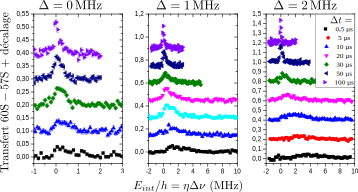
\includegraphics[width=\linewidth]{figures/low_l/expansion_012MHz}
\caption[Spectroscopie microonde de l'expansion du nuage]{
Spectres microonde de la transition $\mathrm{60S-57S}$ au cours de l'évolution d'un nuage de Rydberg excité par un laser désaccordé à $\Delta= 0$ (gauche), $1$ (centre) et $\SI{2}{\MHz}$ (droite).
L'origine des axes verticaux de chacun des spectres est décalée et l'échelle des abscisses et des ordonnées de chacun des graphes est différente, par souci de visibilité.
}
\label{fig:microwave_explosion}
\end{figure}
%
%
\begin{figure}[!h]
\centering
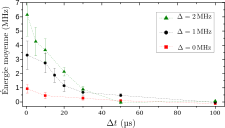
\includegraphics[width=\linewidth]{figures/low_l/energie_moyenne_explosion}
\caption[Énergie moyenne]{
Énergie moyenne
}
\label{fig:avener_explosion}
\end{figure}
%

\newpage
	
		\noindent spectroscopie 60s-57s et son spectre d'excitation : comment cela nous donne accès au spectre des énergies d'interaction\\
		sonder le nuage à différents moments de son explosion

\section{Premier modèle numérique et accord qualitatif}
		\noindent présenter les courbes de Raul.IV.3.2
		
\section{Raffinement du modèle de la dynamique d'excitation}
	\subsection{Simulations}
		\noindent modèle d'équation de taux\\
		\noindent résultats de simulations comparés aux manips\\
	\subsection{Les limites du modèle}
		%\noindent question du chauffage
		\noindent photons thermiques et apparition de niveaux $p$ \\
		LIRE T. PORTO
		
%		
%\section{Spectroscopie microonde du nuage : voir le mouvement}
%	\subsection{Description de la manip}
%		\noindent spectroscopie 60s-57s et son spectre d'excitation : comment cela nous donne accès au spectre des énergies d'interaction\\
%		sonder le nuage à différents moments de son explosion
%	\subsection{Données et accord avec les simulations}
%		\noindent présenter les courbes de Raul.IV.3.2
%		

\section*{Conclusion}
		\noindent il faut prendre en compte le mouvement, mais aussi les transferts thermiques vers les niveaux $p$
		
%\section{Spectroscopie microonde du nuage}
%	\subsection*{Spectre des énergies d'interaction du nuage}
%		\noindent détails sur la spectro 60s-57s, dont la quasi absence de terme d'échange dans l'interaction
%	\subsection*{Mouvement du nuage de Rydbergs}
%		\noindent Le gaz gelé ne marche pas !